% !TEX root =../pfcTipoETSI.tex
\chapter{Ala acuática bidimensional}\LABCHAP{ala2D}
\pagestyle{esitscCD}
\epigraph{ }{}

%\lettrine[lraise=0.7, lines=1, loversize=-0.25]{E}{l} 
\lettrine[lraise=-0.1, lines=2, loversize=0.25]{A}l final del capítulo anterior se expuso la posibilidad de emplear los gradientes favorables de presión se producen en el borde de ataque de un perfil aerodinámico (cuando sobre el incide una corriente con un ángulo de ataque $\alpha$ determinado) como mecanismo para la formación de microburbujas monodispersas, basándose por analogía en los resultados de~\cite{Evangelio2015b}. El objetivo de este capítulo es pues materializar esta idea diseñando, fabricando y realizando experimentos con un dispositivo generador masivo de microburbujas consistente en un perfil aerodinámico\footnote{El diseño de un ala para que pueda realizarse la hipótesis de perfil bidimensional no es trivial, por lo que esta cuestión se abordará con el debido detalle en la \SSEC{DisenoAla}.}. De este modo, se pretende no sólo demostrar que la producción de burbujas de tamaños milimétricos y submilimétricos no lleva necesariamente aparejado el empleo de dispositivos microfluídicos. Además, se contrastarán las hipótesis realizadas en el capítulo anterior y se explorarán las diferentes dificultades que puedan presentarse en el proceso de escalado. 

La estructura que tomará el capítulo será la siguiente: 
\begin{enumerate}
\item En la \SEC{dessign}, se describe todo lo concerniente al diseño y fabricación del modelo completo, que comprende el dispositivo generador de microburbujas y el montaje experimental del mismo. 
\item En la \SEC{experimentos2D}, se especifican los métodos de experimentación y análisis que serán empleados en la obtención de resultados. De este modo, se describirá la configuración final del \textit{set-up}, el protocolo de experimentación, los datos en bruto obtenidos y el posterior tratamiento para el análisis de los mismos.
\item Finalmente, en  la \SEC{results2D}, se muestran y comentan los resultados obtenidos, realizando las conclusiones pertinentes al final del capítulo
\end{enumerate}

\section{Diseño y fabricación}\LABSEC{dessign}

El objetivo de esta sección es describir de forma detallada los parámetros que configuran el diseño del modelo, tanto aquellos que se refieren al dispositivo en sí como al montaje experimental. Para ello, se describen sucintamente en primer lugar los equipos de los que se dispone y las distintas limitaciones de cada uno de ellos, con el fin de poder acotar el diseño final.

\subsection{Equipos disponibles y limitaciones}\LABSSEC{equipos}

La implementación de esta prueba de concepto consistente en un perfil bidimensional implica que la forma más sencilla de crear una corriente relativa entre el fluido y el perfil sea fijando este último y haciendo incidir sobre él un líquido a la velocidad uniforme $U_{\infty}$; esta implementación puede realizarse perfectamente en un túnel hidrodinámico. Por otro lado, se precisará de un sistema de inyección de aire que permita la formación de las burbujas, por lo que se requiere una linea de presión acompañada de manorreductores que permitan abordar esta tarea. Finalmente, para poder obtener y posteriormente analizar los datos extraídos del experimento, será necesario poder documentarlo, para lo cual se hará uso de una cámara de vídeo. Esta cámara no puede ser cualquiera, ya que el fenómeno que se pretende grabar ocurre en unas pocas fracciones de segundo. En efecto, si se pretenden obtener con este dispositivo burbujas de tamaños comparables a las encontradas en~\cite{Evangelio2015b}, esto es $d_{b}\sim \mathcal{O}\left(200\,\mathrm{\mu m}\right)$, y se estima que las burbujas son convectadas aguas abajo del perfil a una velocidad\footnote{En~\cite{Evngelio2015b}, las burbujas son convectadas a la velocidad de la corriente, siendo en este caso $U$ la velocidad media en el capilar para $Re \gg 1$.} $v \sim U_{\infty}$, se tendrá que una burbuja recorre una distancia del orden de su diámetro en un tiempo $t_{b} \sim d_{b}/U_{\infty} \sim \mathcal{O}\left(200\,\mathrm{\mu s}\right)$, por lo que serán necesarios del orden de 5000~fotogramas por segundo (en adelante fps): se necesita, por lo tanto, una cámara de alta velocidad. 

\subsubsection*{Tunel hidrodinámico}

En el laboratorio de Mecánica de Fluidos de la Escuela Superior de Ingeniería de Sevilla se dispone de un túnel hidrodinámico como el mostrado en la \FIG{tunel}. Como puede observarse en la figura, el túnel consiste en un conducto de sección rectangular a través del cual se hace circular un líquido (en este caso agua) utilizando para ello una bomba. Una vez que la bomba ha hecho ascender al líquido hasta la altura adecuada, se le hace pasar a través de una cámara de contracción cuyo fin es uniformizar el flujo incidente en la cámara de ensayos (zona transparente del túnel). Pese a no apreciarse en la imagen, el túnel se encuentra abierto  y en contacto con la atmósfera en su parte superior, mientras que la parte inferior del mismo también esta formada por cristales de igual transparencia que las paredes laterales. Las dimensiones del túnel pueden consultarse en la \TAB{tunel}

\begin{table}
\begin{tabular}{c c}
\textbf{Dimensión} & Valor [cm] \\
\hline \hline
Ancho de la sección & slka  \\
Altura de la secció & sajfios \\
distancia entre soportes & fljisd \\
\hline
\end{tabular}
\caption{Dimensiones relevantes del túnel hidrodinámico}
\LABTAB{tunel}
\end{table}

\begin{figure}
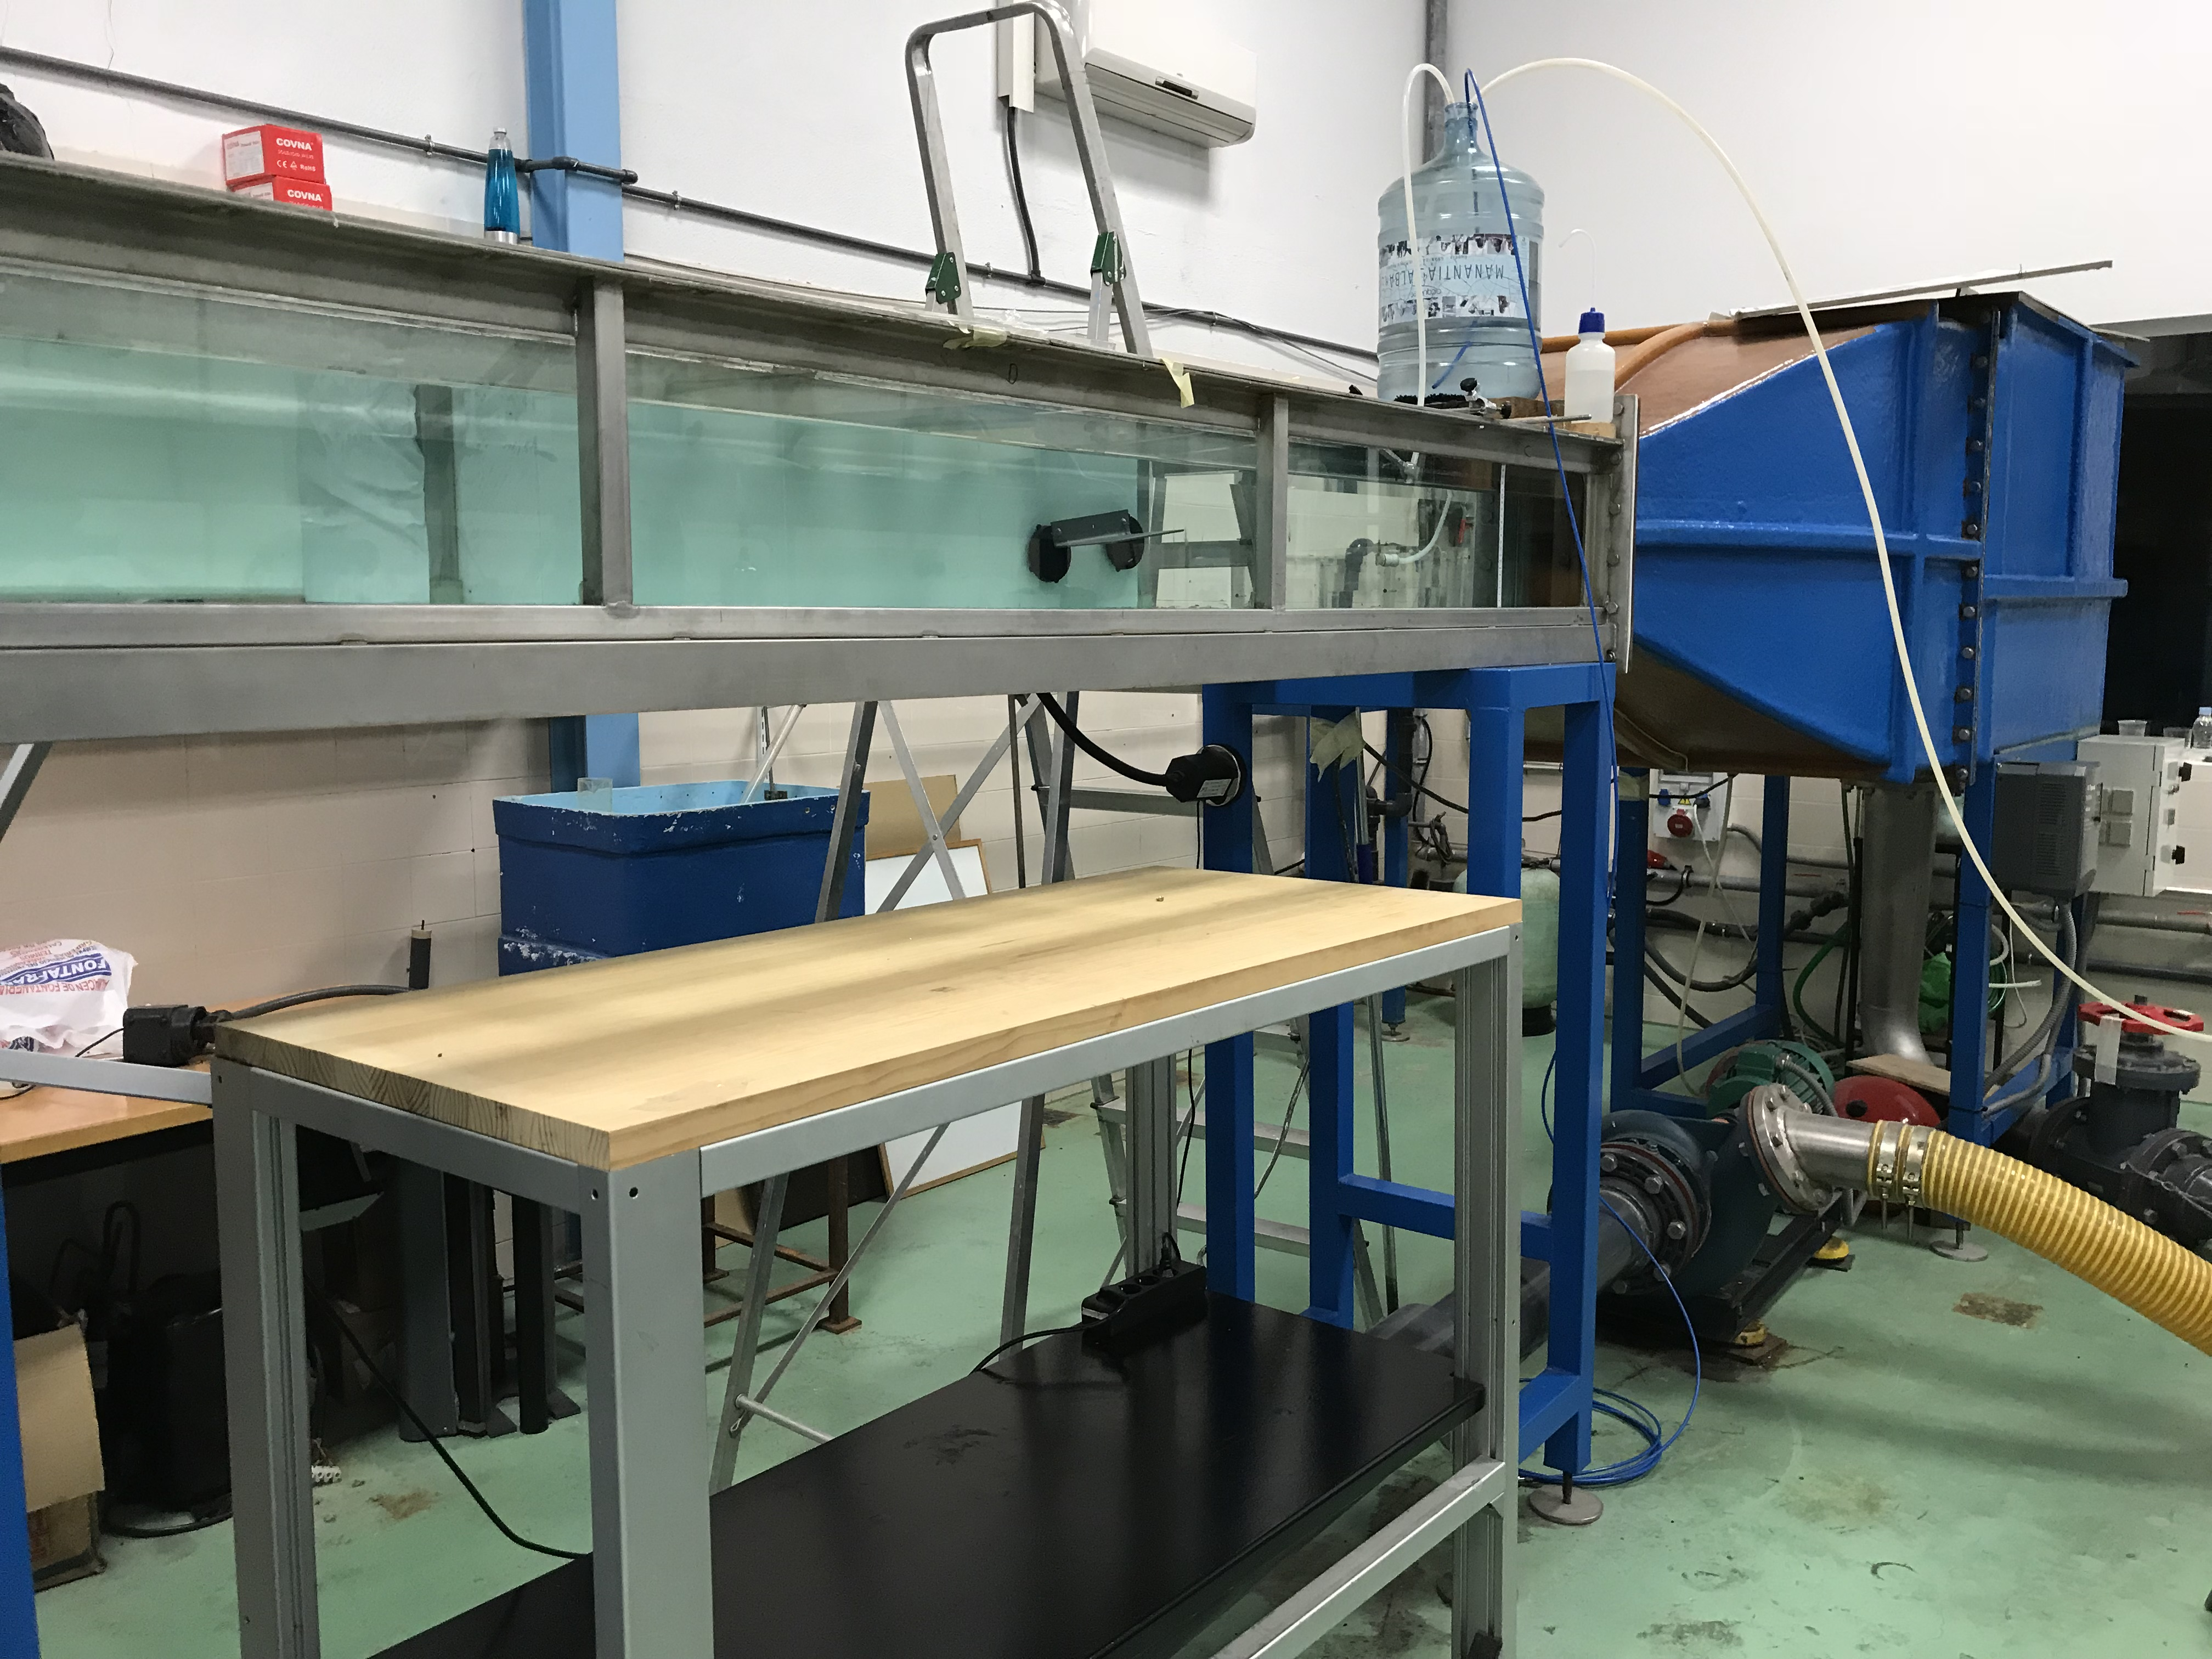
\includegraphics[scale=1]{ala2D/figuras/tunel.jpg}
\caption{Perspectiva del túnel hidrodinámico donde los experimentos han sido realizados.}
\LABFIG{tunel}
\end{figure}

Para el control del caudal que circula a través del túnel hidrodinámico se disponen de dos grados de libertad: la altura total del agua (esto es, la fracción de la sección del túnel que queda mojada) y la velocidad media del agua en la sección. Dado que el túnel se encuentra abierto en su parte superior, se ha comprobado experimentalmente que la velocidad del túnel no puede excederse por encima de $U_{\infty} \sim 0.75\,\mathrm{m/s}$ si se quiere evitar la formación de ondas superficiales. Por lo tanto, se tomará como restricción al diseño que la velocidad de la corriente incidente no puede superar este valor, es decir,

\begin{equation}
U_{\infty} \leq 0.75\,\mathrm{m/s}
\LABEQ{restrVel}
\end{equation}

Finalmente, cabe destacar que el control de la velocidad del túnel se realiza a través de un regulador de potencia, por lo que la medida de la velocidad para cada potencia debe determinarse experimentalmente. 

\subsubsection*{Reguladores de presión}

La formación de burbujas requerirá que se inyecte aire en ciertos puntos de la superficie del ala, el cual debe proceder desde dentro de la misma. Para poder suministrar aire se dispone de una red de presión capaz de suministrar más de 6 bares de presión, lo cual es más que suficiente para el propósito que nos ocupa. Para regular de forma adecuada la presión se dispone de manorreductores cuya precisión es de 1~mbar. 

\subsubsection*{Cámara de alta velocidad}

Se dispone de una cámara Phantom~v710 como la que se muestra en la \FIG{phantom}, capaz de grabar a más de 1~millón de fps. Dado que, según se comentó al inicio de esta sección, serán necesarios en torno a 5000~fps, esta cámara es capaz de acometer dicha tarea sin problema alguno.  Adicionalmente, se disponen de dos objetivos Canon\textsuperscript{\textregistered} diferentes  con zoom 1-4 y 2.5-10, respectivamente. Finalmente, cabe destacar que la distancia focal de la cámara es de aproximadamente 11~cm.


\subsection{Diseño del ala}\LABSSEC{disenoAla}

Una vez que se consideran los equipos disponibles y las restricciones que pueda imponer cada uno, es momento de pasar a especificar el diseño final del ala. Dado que la sección transversal del ala consiste en un perfil aerodinámico, se ha decidido que el proceso de fabricación sea mediante control numérico, empleando un polímero de ABS (Acrilonitrilo Butadieno Estireno, de sus siglas en inglés) como materia prima. La fabriación por control numérico aúna las ventajas de la impresión~3D y la fabricación tradicional, ya que las paredes de la pieza obtenidas son siempre macizas\footnote{Mediante impresión 3D también es posible emplear un 100\% de entramado, con lo que se obtendrían resultados parecidos con el mismo material; si bien, el empleo de la técnica de impresión 3D con entramados tan elevados suele llevar aparejado un alto coste.} lo que aportará la robustez necesaria para soportar la experimentación del ala en el agua del túnel hidrodinámico.

Para la sección transversal del ala se disponen de dos opciones principales en lo que a perfiles aerodinámicos se refiere: o bien se opta por diseñar un perfil personalizado, o bien se emplea alguno de los perfiles normalizados ya existentes, por ejemplo los de la serie NACA. Se ha elegido para este primer prototipo el conocido perfil simétrico NACA~0012, que posee un espesor máximo relativo a la cuerda $t/c\ = 0.12$. El motivo de empleo de un perfil de estas características se basa principalmente en que el NACA~0012 es uno de los perfiles aerodinámicos más estudiados, lo que unido a la sencillez en su diseño lo hacen idóneo para una primera prueba de concepto. No obstante, el empleo de un perfil con curvatura no supondría una pérdida de generalidad en los resultados obtenidos adelante.

Decidido el perfil aerodinámico que se empleará como sección transversal del ala, tan sólo es necesario definir la cuerda, $c$, y la envergadura, $b$, para tener completamente definida la geometría exterior del ala. Para la cuerda es necesario tener en cuenta los puntos de sujeción que tendrá el ala dentro del túnel hidrodinámico. En principio, podría optarse por disponer de 2 únicos puntos de sujeción (uno a cada lado del ala) que fueran acoplados en torno a una distancia $c/2$ del borde de ataque. Sin embargo, dado que en los experimentos se pretende variar el ángulo de ataque de la corriente inicidente, el diseño de un sistema capaz de variar la inclinación del ala con sólo 2 puntos de sujeción es bastante complejo. Por ello, resulta más sencillo disponer de 4 puntos de sujeción, de forma que se sitúen 2 de ellos cerca del borde de ataque y otros dos cerca del borde de salida, permaneciendo los primeros fijos durante la operación experimental, lo que permite variar la inclinación del ala y con ello el ángulo de ataque $\alpha$ con el que inicide la corriente. El valor que toma la cuerda, de este modo, debe ser tal que permita que el ala se sitúe entre 2 puntos de soporte consecutivos del túnel (véase la \TAB{tunel}), por lo que se ha decidido darle un valor $c = .3\,\mathrm{m}$. En este momento, elegida la magnitud de la cuerda,   se está en condiciones de poder calcular el número de Reynolds global en el ala, 

\begin{equation}
Re_{c}  = \dfrac{\rho U_{\infty} c}{\mu} \sim \mathcal{O}\left(10^{5}\right) \gg 1. 
\end{equation}

donde se ha tomado un valor orientativo $U_{\infty} \sim 0.5\,\mathrm{m/s}$. Por lo tanto, la magnitud de la cuerda escogida permite sin mayor complicación disponer de las condiciones de $Re_{c} \gg 1$ tal y como se pretendía. El cálculo del valor adecuado que se debe dar a la envergadura, por otro lado, sigue un razonamiento diferente. Modelar experimentalmente un problema bidimensional no es una tarea fácil en la mayoría de los campos de la física, ya que se deben asegurar el cumplimiento de las hipótesis que con el fin de simplificar el problema base se hayan realizado. Como se comentó en la \SEC{aerodynamics}, para el caso de el movimiento de un sólido fuselado en el seno de un fluido incompresible a altos números de Reynolds tal que el flujo inicialmente es irrotacional, se obtiene el problema descrito por las ecuaciones \eqref{eq:problemaContorno}. La linealidad del problema de contorno especificado, admite que pueda ser resuelto mediante superposición de soluciones elementales de la laplaciana, como son los términos fuente (y/o sumideros), los torbellinos y los dobletes. % AÑADIR AQUI SI PROCEDE REFERENCIAS ADECUADAS AL MÉTODO DE CONTORNO DEL LIBRO DE AERODINÁMICA
Por otro lado, cuando existen contornos rígidos como una pared, la teoría de campos permite emplear el \emph{método de las imágenes}, que consiste en aplicar una simetría en la distribución de soluciones elementales respecto al contorno en cuestión de forma que se cumplan las condiciones de contorno en la pared (en este caso, $\nabla \phi \cdot \mathbf{n} = 0$), lo que permite modelar el efecto que la pared ejerce sobre el campo potencial solución del problema respecto al campo original. De este modo, este mismo razonamiento puede ser empleado de forma inversa: para modelar un perfil aerodinámico bidimensional, se tendría que disponer de un ala \emph{infinitamente} larga, de modo que los torbellinos de la punta no indujeran velocidades transversales a la corriente incidente\footnote{Este aspecto pertenece a la teoría de alas de envergadura finita, cuya descripción detallada puede encontrarse en el \CHAP{ala3D}  y  en el %PONER AQUI EL APENDICE PARA ALAS 3D
} y por tanto perpendiculares al plano del problema 2D, rompiendo así la hipótesis de bidimensionalidad. Gracias al método de las imágenes, es posible modelar este  comportamiento si se empotra el ala en las paredes del túnel, para lo cual la envergadura del ala tendría que coincidir con el ancho de la sección. Sucede sin embargo que las paredes del túnel son de cristal, lo que imposibilita la opción de atornillar o taladrar en ellas la sujeción del ala, de modo que se empleará una envergadura ligeramente inferior que permita un sistema alternativo de sujeción, descrito en la \SSEC{disenoSetup}; nótese que, al no poder aplicar estrictamente el método de las imágenes, se está realizando pues la hipótesis de comportamiento bidimensional, que tendrá que ser corroborada \textit{a posteriori}. El valor empleado de la envergadura es pues $b = lo que sea$.

Hasta este punto se tiene completamente definida la geometría exterior del ala, pero aún no posee las condiciones para poder generar burbujas. Como ya se comentó previamente, el aire debe inyectarse a través de determinados orificios de la  superficie del ala, por lo que el gas debe provenir directamente desde dentro de la misma. Para ello, se disponen de dos posiblidades. Una sería llevar el aire  desde un depósito situado en el exterior del túnel a través de conductos (como son los tubos de \emph{tygon} o tubos de \emph{peek}) hasta cada orificio, lo que sería directo pero complicaría el diseño, al tiempo que requeriría un sellado muy meticuloso de la zona de intersección de los tubos con el ala. La otra, sería convertir el propio ala en un depósito, para lo cual simplemente habría que diseñar el dispositivo de forma que fuera hueco por dentro. Esta última opción es la que se ha elegido, pudiéndose observar en la \FIG{seccionAla} un corte longitudinal en perpsectiva donde se aprecia la oquedad interior. Así, a través de  un orificio roscado con, un racor adaptará el interior del ala a la red de presión disponible. 

\begin{figure}
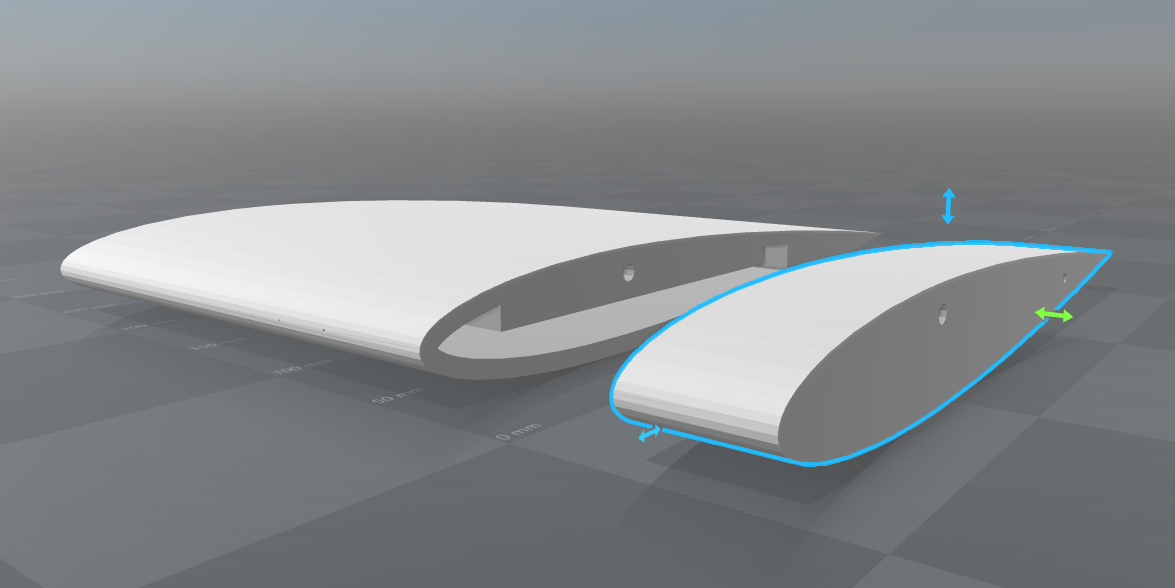
\includegraphics[scale=1]{ala2D/figuras/seccionAla.jpg}
\caption{Perspectiva de la sección longitudinal del dispositivo generador de microburbujas. En la figura puede apreciarse el interior hueco del ala que se hallará presurizado para poder suministrar el caudal de gas requerido. }
\LABFIG{seccionAla}
\end{figure}

Para concluir el diseño del sistema de inyección de aire, es necesario indicar los puntos donde se situarán los orificios a través de los cuales el aire será introducido en el líquido. Recordando las conclusiones extraídas en el capítulo anterior, resulta evidente que los orificios deben situarse en las zonas donde el gradiente favorable de presión sea mayor, esto es, la región que, conteniendo al borde de ataque, se encuentra entre el punto de remanso y el pico de succión del perfil. No obstante, la posición de sendos puntos no es fija, sino que depende (para un perfil simétrico) depende del ángulo de ataque de la corriente incidente, por lo que parece conveniente distribuir los puntos de inyección en un entorno del borde de ataque y sobre una misma superficie del perfil (extradós o intradós), que será donde se grabe el proceso de formación de burbujas. De este modo,en cada punto y para cada $\alpha$, se tendrán distintos valores del gradiente de presión adimensional, $\mathrm{d}\,c_{p}/\mathrm{d}x$. Cabe apreciar además, que puede darse la circunstancia de que, para determinados valores de $\alpha$, los puntos pasen de encontrarse en una zona de gradiente favorable de presión a una zona de gradiente desfavorable de presión, o lo que es lo mismo, aguas abajo del pico de succión. En la \TAB{orificios} se muestran las posiciones adimensionalizadas con la cuerda de la abcisa de los puntos de inyección tomando $x$ según el eje longitudinal de simetría del perfil con origen en el borde de ataque (\FIG{airfoil})


\begin{table}
\centering
\begin{tabular}{c || c c c c c c c}
\textbf{Puntos} &1&2&3&4&5&6&7 \\
\hline \hline
$\mathbf{x/c}$ & 1 &2 &3 &4 &5 &6 &7 \\
\end{tabular}
\caption{Posición de la abcisa, adimensionalizada con la cuerda del perfil, de los orificios de inyeccón de aire.}
\LABTAB{orificios}
\end{table}

Finalmente, en lo que se refiere al diámetro y longtiud del los orificios, se debe tener en cuenta que resulta primordial asegurar la constancia del caudal durante el experimento, lo que no será trivial si se tienen en cuenta las perturbaciones que puedan existir tanto en la presión dentro del ala como en la presión en el otro extremo del orificio (al agua bordeando el perfil). Para minimizar las variaciones de caudal causadas por las perturbaciones de presión y con idea de poder efectuar variaciones graduales de caudal mediante una variación mínima de presión de 1~mbar (precisión de los manorreductores), la solución que se propone es el empleo de tubos capilares que generen una gran pérdida de carga. En efecto, si se asume que el flujo en el interior del tubo capilar es tal que $Re_{D}\,D/L_{t} \ll 1$,\footnote{Esta hipótesis podrá ser comprobada una vez se analicen los resultados en la \SEC{resultados2D}} con $Re_{D} =  4Q_{g}/\left(\pi D \nu \right)$ el número de Reynolds basado en el diámetro del tubo $D$ y $L_{t}$ la longitud del mismo, el flujo de gas por el interior del tubo es casi-unidireccional y sigue la ley de Hägen-Poiseuille,

\begin{equation}
Q_{g} = \dfrac{\pi D^{4}}{128 \mu_{g}}\dfrac{\Delta p}{L_{t}}
\LABEQ{poiseuille}
\end{equation}

donde $\Delta p$ es el incremento de presón entre el interior y el exterior del ala. Si se llama ahora $\delta p$ a la perturbación en el incremento de presión, se tiene que el incremento de presión total será $\Delta p = \Delta p_{0} + \delta p$, que provocará un flujo de air total igual a 

\begin{equation}
Q_{g} = Q_{g_{0}} + \delta Q_{g} = \dfrac{\pi D^{4}}{128 \mu_{g} L_{t}}\left(\Delta p_{0} +  \delta p\right) \Rightarrow \delta Q = \dfrac{\pi D^{4}}{128 \mu_{g} L_{t}}\delta p = \dfrac{\pi D^{3}}{128\mu_{g}}\dfrac{D}{L_{t}}\delta p
\LABEQ{perdidaCarga}
\end{equation}

Por lo tanto, según la \EQ{perdidaCarga}, se tiene que las perturbaciones en los incrementos de presión provacarán incrementos de caudal más pequeños cuanto menor sea el díametro $D$ y el cociente $D/L_{t}$. De este modo, para que la inyección de aire a caudal constante sea lo más estable posible, se hace necesario reducir todo lo posible el diámetro del orifiio de salida. Así pues, considerando las limitaciones tecnológicas existentes para perforar un orificio del tamaño de, por ejemplo $200\,\mathrm{\mu m}$, la mejor alternativa resulta en utilizar tubos capilares con el diámetro interior que se requiera y un diámetro exterior más manejable que permita su inclusión dentro de los orificios del ala. Para el prototipo que se está describiendo, se han empleado tubos capilares de acero con diámetro exterior $D_{ext} = 400\,\mathrm{\mu m}$ y diámetro interior $D = 160\, \mathrm{\mu m}$. 

Para concluir esta sección, se muestran en la \FIG{ala2DFinal} diferentes perspectivas del aspecto final del dispositivo generador de microburbujas descrito hasta este punto. Nótese la presencia en los extremos laterales del ala de un orificio pasante cerca del borde de ataque así como otro ciego cerca del borde de salida: estos orificios, que forman parte del sistema de variación del ángulo de ataque, serán descritos en detalle y por conveniencia dentro de la \SSEC{disenoSetup}. 

\begin{figure}
\centering
\subfloat[Perspectiva 1]{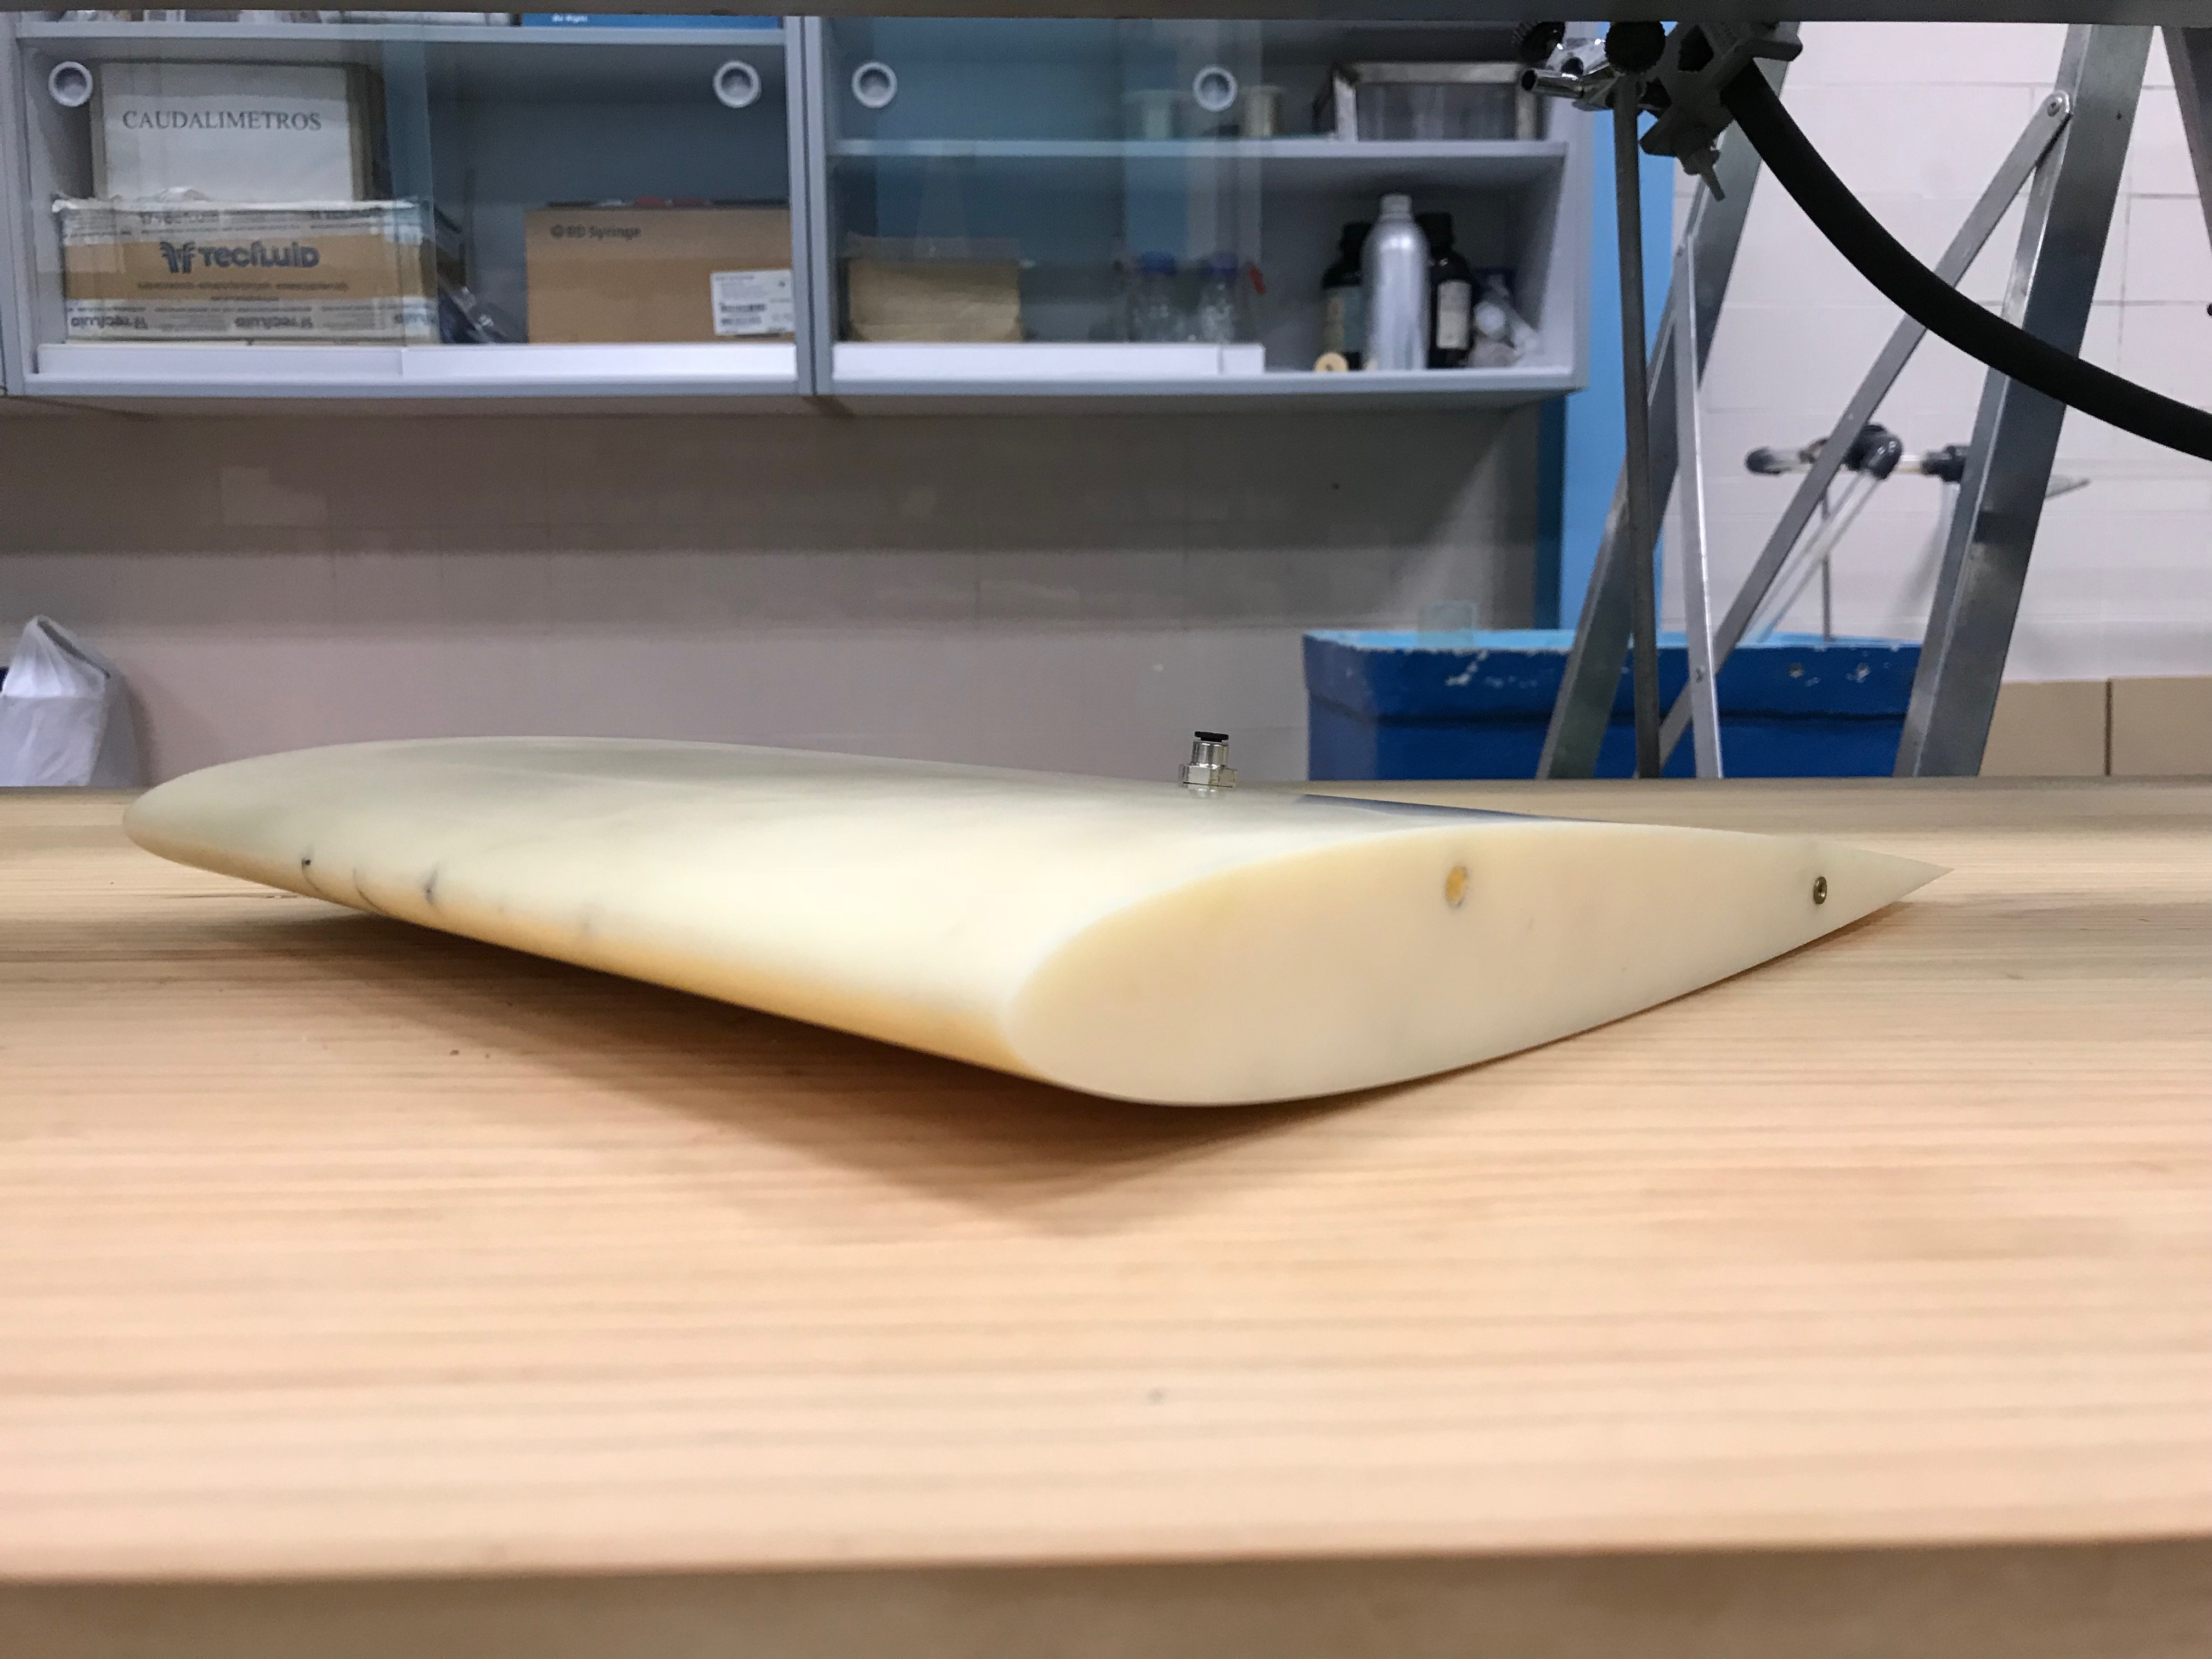
\includegraphics[width = .5\textwidth]{ala2D/figuras/ala2D_1.jpg}}
\subfloat[Perspectiva 2]{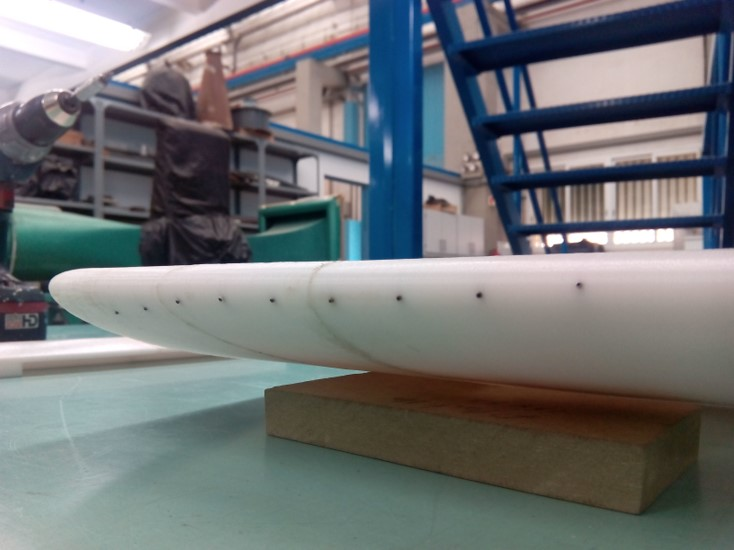
\includegraphics[width = .5\textwidth]{ala2D/figuras/ala2D_2.jpg}}
\caption{Diferentes perspectivas del dispositivo generador de microburbujas bidimensional empleado en los experimentos.}
\LABFIG{ala2DFinal}
\end{figure}



\subsection{Diseño del montaje experimental}\LABSSEC{disenoSetup}

Una vez ya se tiene completado el diseño y la fabriación del ala, tan sólo queda crear un montaje adecuado para poder realizar los experimentos. El primer objetivo de este montaje será un sistema capaz de no sólo posicionar el ala dentro del túnel hidrodinámico sino también de poder variar el ángulo de ataque, $\alpha$. En la \FIG{estructuraAluminio} puede observarse que la estructura consta de los sigiuentes componentes:

\begin{itemize}
\item Dos largeros longitudinales, los cuales sirven para anclar la estructura a los tornillos que sobresalen en la parte superior del túnel, de forma que la unión con este sea lo más robusta posible. 
\item Dos largeros anteriores verticales, que ejercen  la función de puntos de sujeción del ala cerca del borde de ataque. Estos largueros, que deben estar completamente en contacto con las paredes laterales del túnel,  poseen orificios que permiten en paso del eje que recorre transversalmente al ala y que forma parte del sistema de variación del ángulo de ataque.
\item Dos largueros transversales, de los cuales el situado en la parte delantera (cerca del borde de ataque del ala) sirve para dar robustez a la estructura, mientras que el trasero (además de proveer estabilidad), incluye el sistema de variación del ángulo de ataque.
\end{itemize}


El sistema de variación del ángulo de ataque, por lo tanto, funciona del siguiente modo: un eje metálico  pasa a través del orificio pasante del ala cerca del borde de ataque (véase la \FIG{ala2DFinal}), desembocando en las ranuras practicadas en los largueros verticales, con lo que el único grado de libertad no impedido del ala es el giro alrededor de dicho eje; por otro lado, en su parte posterior, dos varillas atornilladas cerca del borde de salida sujetan el ala al larguero transversal trasero, pasando cada varila a través de un espárrago que fija la posición de las mismas con un tornillo de teflón (este tipo de tornillo permite fijar la posición de las varillas sin perforarlas o dañarlas). 


\begin{figure}
\centering
\includegraphics[scale=1]{ala2D/figuras/estructuraAluminio.jpg}
\caption{Estructura de aluminio emplead como sistema posicionador del ala dentro del túnel hidrodinámico. En su parte posterior, los largerillos incluyen dos cilindros que permiten el paso de las varillas que permiten regular la inclinación del ala.}
\LABFIG{estructuraAluminio}
\end{figure}


Una vez el ala es fijada dentro del túnel, para completar el montaje se debe instalar el equipo de visualización. En la \FIG{setupCompleto}, donde puede apreciarse todo el montaje experimental completo, se muestra en qué consiste el equipo de visualización: la cámara de alta velocidad descrita en la \SSEC{equipos} es instalada de forma vertial a un sistema de posicionadores que permite cambiar la posición de la cámara de forma muy precisa; además, se dispone de una lámpara de luz fría que mediante un tubo de fibra óptica permite iluminar adecuadamente la zona que se desea documentar. La presencia de la superficie libre en la zona superior del túnel hace que la visualización desde dicha zona sea imposible, por lo que debe grabarse en vertical desde abajo. 


\begin{figure}
\centering
\subfloat[Montaje del ala en el túnel]{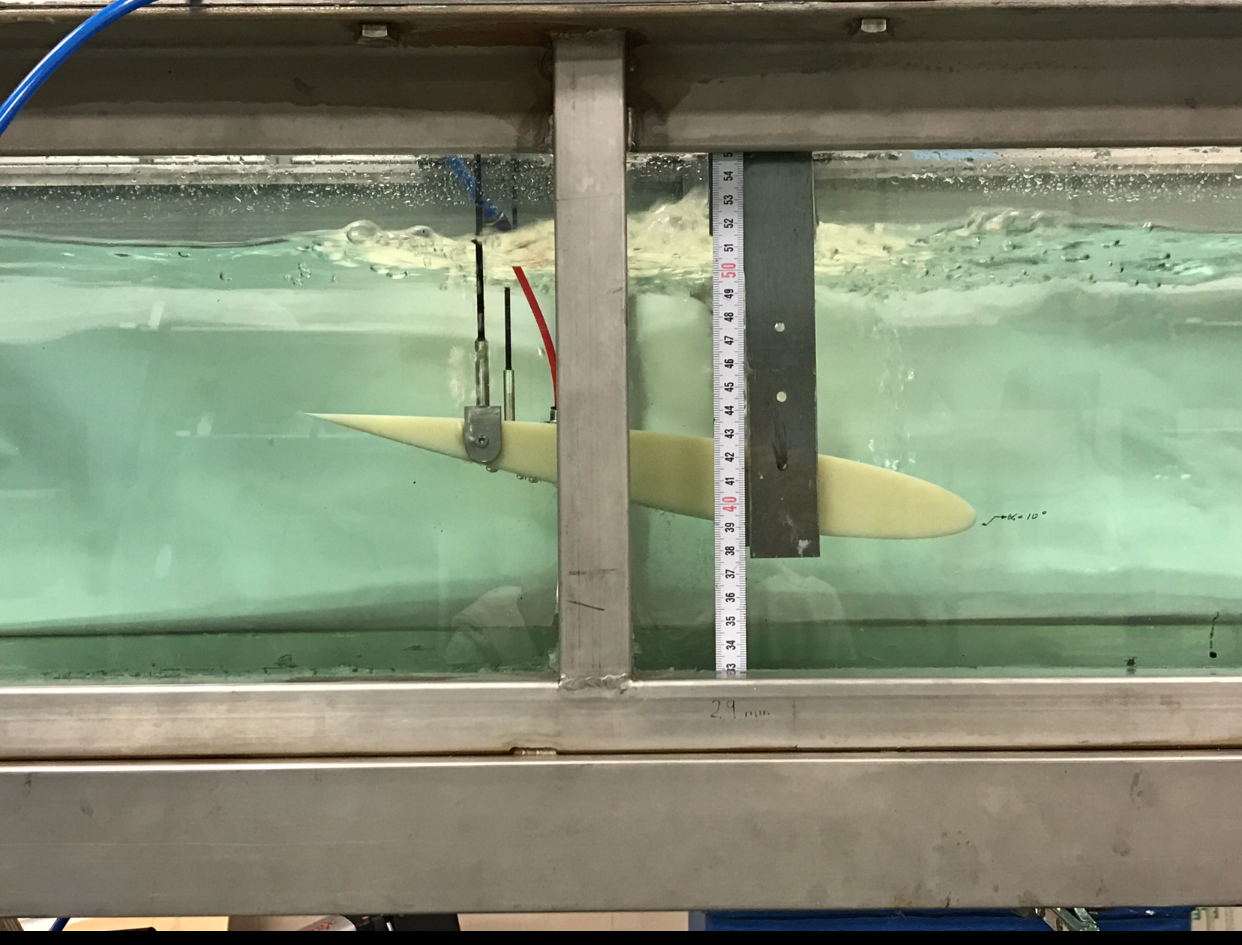
\includegraphics[width = .5\textwidth]{ala2D/figuras/montajeAla.jpg}\LABFIG{montajeAla}}
\subfloat[Equipo de visualización]{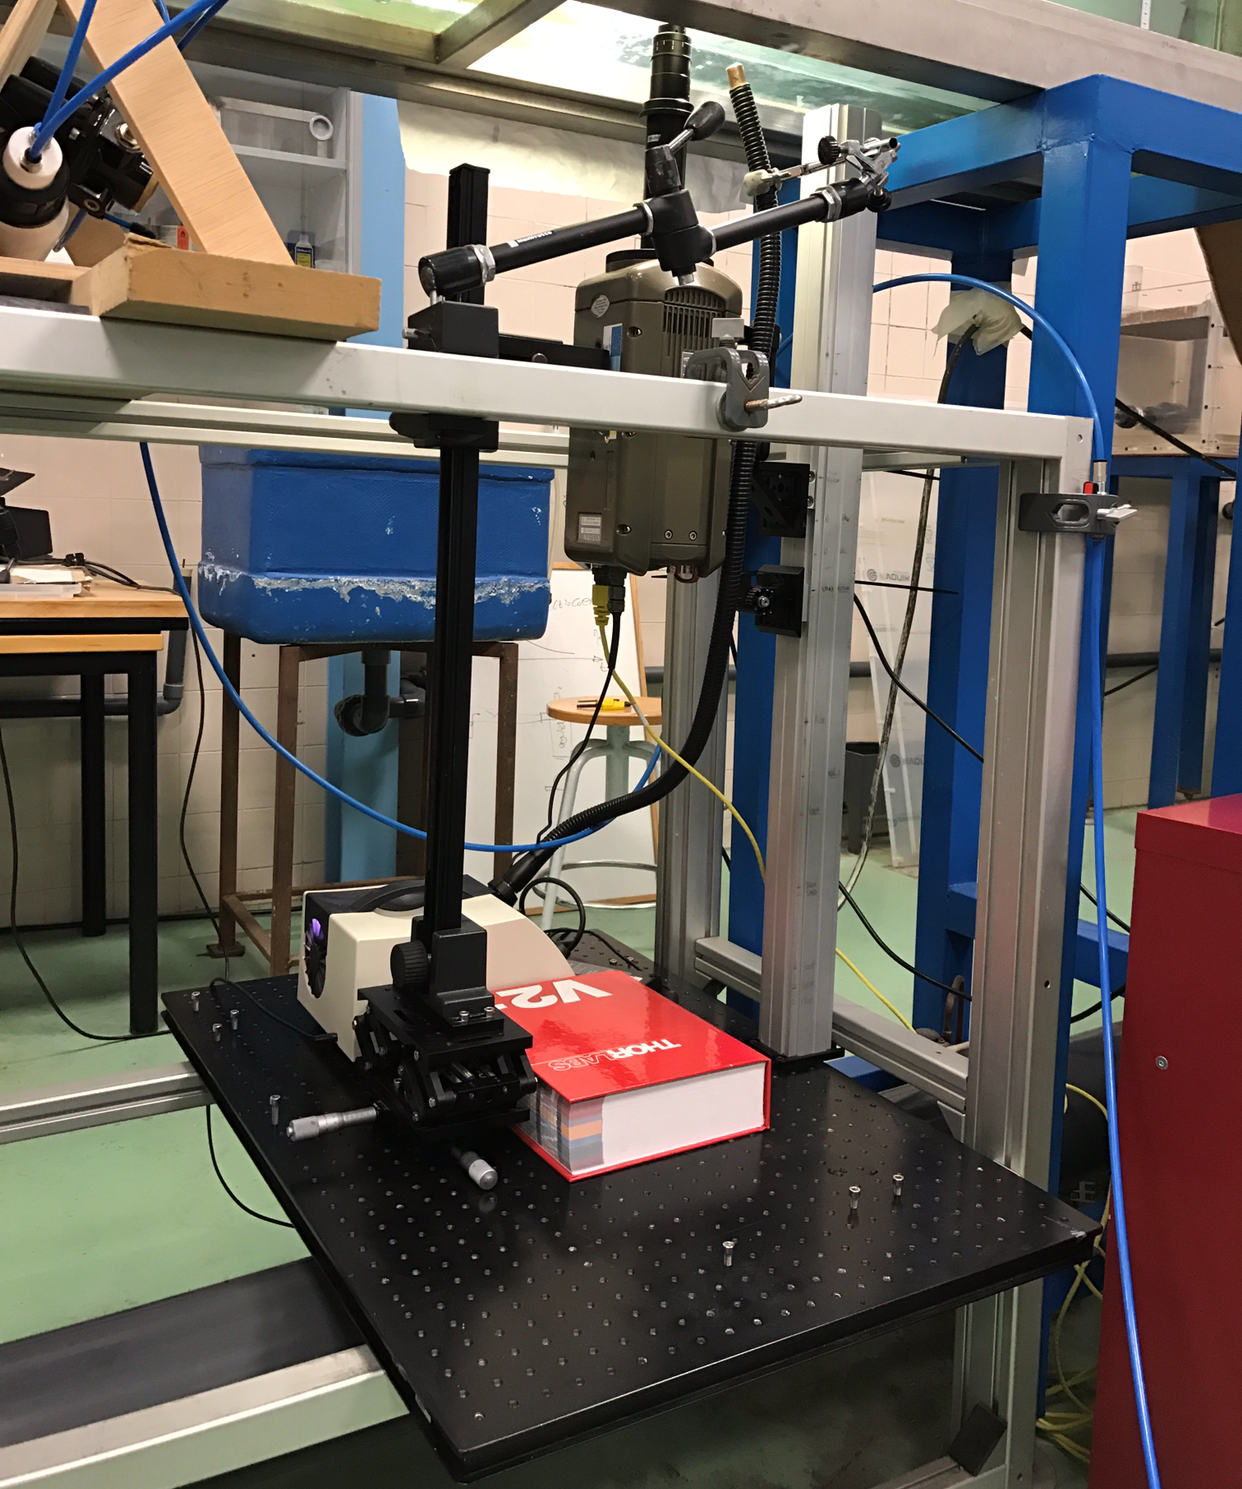
\includegraphics[width = .5\textwidth]{ala2D/figuras/visualizacion.jpg}\LABFIG{visualizacion}} \\
\subfloat[Montaje experimental completo]{\includegraphics[width = \textwidth]{ala2D/figuras/setupCompleto.jpg}\LABFIG{setup}}
\caption{Montaje experimental completo. En la \FIG{montajeAla} puede apreciarse el sistema de posicionamiento del ala y variación del ángulo de ataque mientras que en la \FIG{visualizacion} se muestra el equipo de visualización. La \FIG{setup} muestra una perspectiva del montaje experimental.}
\LABFIG{setupCompleto}
\end{figure}


\section{Experimentos}\LABSEC{experimentos}

Tras el recorrido realizado a través del proceso de diseño y fabriación de este dispositivo generador de burbujas, es el momento de testearlo con una exhaustiva campaña experimental. En esta sección se muestran todos los detalles concernientes al experimento, tales como los parámetros que se han empleado y el rango en el que estos han variado, así como el protocolo seguido durante una serie experimental. Finalmente, para concluir la sección, se especifican cuáles son los datos en bruto frutos del proceso experimental y en cuáles son los métodos empleados para el procesado de dichos datos, cuyos resultados serán mostrados en la siguiente sección. 

\subsection{Campaña experimental}\LABSSEC{campExperimental}

Atendiendo a los resultados hallados en~\cite{Evangelio2015} y resumidos en la \SEC{gradPres}, el diámetro y frecuencias de las burbujas producidas dependerá, dada una geometría fija, del caudal de gas inyectado, la velocidad del líquido exterior y  del gradiente de presión local adimensionalizado en el punto de formación de la burbuja. Son estos, por lo tanto, las tres variables que configuran el espacio paramétrico que debe ser testeado en los experimentos.  En la \TAB{parametros2D} se muestran los valores empleados de estos tres grados de libertad para los diferentes experimentos; nótese que, dado el montaje realizado, no se puede controlar directamente el valor del caudal, ya que este depende de la diferencia de presión entre el interior y el exterior del ala, siendo esta última variable con la velocidad y el ángulo de ataque. Por lo tanto, se toma como variable libre el valor de la presión interior del ala, debiendo calcularse el caudal de gas inyectado \textit{a posteriori}. Conviene destacar los siguientes aspectos de los valores de la tabla:

\begin{itemize}
\item Los valores de la velocidad inicidente son determinados, como ya se especificó, de forma indirecta, ya que el regulador de potencia del túnel no permite controlar directamente la velocidad. Los detalles del sistema de medición de velocidad se especifcan más adelante en la \SSEC{metodos}.
\item Los valores de la presión interior del depósito fueron fijados durante una de las primeras pruebas experiemntales, comprobando cuándo se producían variaciones significativas en los diámetros de las burbujas al variar la presión interior del ala manteniendo la velocidad y el ángulo de ataque constantes. 
\item Los valores del ángulo de ataque que figuran en la \TAB{parametros}, han sido calculados \textit{a posteriori } según los métodos especificados más adelante. Los valores orientativos del ángulo de ataque que se pretendían conseguir varían entre $4-12^{\circ}$ cada $2^{\circ}$. Cabe decir que no se consideraron valores $\alpha > 12^{\circ}$ con el fin de estar suficientemente lejos de los valores que propiciarían el desprendimiento de la capa límite. 
\end{itemize}


\begin{table}
\centering
\begin{tabular}{c || c c c}
\textbf{Parámetros} & $U_{\infty}\,\left[\mathrm{m/s}\right]$ & $P_{int}\,\left[mbar\right]$ & $\alpha\,\left[^{\circ}\right]$  \\
\hline \hline
\textbf{Valores} & 0.3,0.5,0.6,0.72 & 120,289,400,520,650,789 & 4.66, 6.11, 8.5, 10, 12 \\
\hline
\end{tabular}
\caption{Rango paramétrico empleado durante la realización de los experimentos.}
\end{table}

Por otro lado, para la grabación de imágenes a alta velocidad, cabe destacar que se ha empleado una resolución %tanto x tanto
grabando a una velocidad de % No me acuerdo cuantos
fps. Así pues, habiendo especificado tanto los valores entre los que variarán los parámetros del experimento como las concidicones de grabación, se puede describir cuál es el protocolo que permite la obtención de datos de una serie experimental (esto es, una combinación de la terna $\left[Pint,U_{\infty},\alpha\right]$), de modo que sirva de ejemplo del proceso completo de obtención de los datos que serán procesados en la siguiente sección. 

El protocolo de experimentación seguido busca efectuar los realizar los ensayos de la forma más rigurosa y eficiente posible, optimizando los tiempos requeridos para cada tarea. Una ves se tiene el ala fijada en el túnel hidrodinámico, el circuito de presión conectado al ala con una presión arbitraria (pero lo suficiente para evitar que entre agua a través de los orificios) y el sistema de visualización correctamente configurado y enfocado, se procede del siguiente modo:

\begin{enumerate}
\item Se fija el ángulo de ataque, $\alpha$, deseado para dicho experimento. Para ello se deben mover las varillas hasta encontrar (ayudándose de un transportador) aproximadamente el ángulo buscado y posteriormente fijarlas.
\item Una vez encontrado el ángulo de ataque, se toma una fotografía de la forma más ortogonal posbile de la sección transversal del ala. Dicha imagen será utilizada para calcular el ángulo de ataque real con el que incide la corriente.
\item En este punto, si fuera necesario, se vuelve al paso~1 hasta encontrar un valor aproximado al esperado para $\alpha$.
\item Fijado el valor de $\alpha$, se selecciona la velocidad a la que se realizará el ensayo.
\item Finalmente, se selecciona una presión interior de las encontradas en la \TAB{parametros} y se deja transcurrir un tiempo suficiente hasta alcanzar un régimen estacionario\footnote{Durante la operación experimental este tiempo podía consistir en 20-30s, que es el tiempo que se tardaba en configurar y prepara el video para la grabación. En la \SEC{resultados2D} se comprobará como este tiempo es mucho mayor que el tiempo de difusión viscosa $D^{2}/\nu_{g}$ o el tiempo característico que emplea el gas en recorrer el tubo capilar.}.
\item Se configura la cámara para que inicie la grabación y se toman 3 vídeos de 3 instantes diferentes con la intención de poder realizar una media de los valores obtenidos.
\item Mientras se produce la grabación de los videos, se regula la presión para poder continuar con el siguiente valor.
\item Finalizadas todas las pruebas variando la presión interior del ala y manteniendo la velocidad y el ángulo de ataque constantes, se  procede a cambiar el valor de la velocidad y repetir los pasos 5-7, y así hasta completar todas las velocidades. 
\item Finalmente, si se desea, se modifica el valor del ángulo de ataque y se repiten los pasos anteriores.

\end{enumerate}


\subsection{Datos obtenidos y métodos de postproceso}\LABSSEC{metodos}

Llegados a este punto y concluidos todos los experimentos, se dispone de un material en bruto que requiere un meticuloso postproceso para su posterior análisis. Es objeto de esta sección detallar los métodos que se han utilizado para llegar a los resultados mostrados en la \SEC{resultados2D}. 

\subsubsection*{Videos}

Fruto de los ensayos realizados se dispondrá de 3 vídeos para cada terna de parámetros $\left(\alpha, U_{\infty}, P_{int}\right)$. Un ejemplo ilustrativo del tipo de imágen que se obtiene de la grabación con la cámara de alta velocidad puede encontrarse en la \FIG{ejemploVideo2D} donde se muestra la producción de burbujas en un orificio situado en el borde de ataque. Debido a que se dispone de distancias calibradas en la imagen, es imediato realizar la medición de los diámetros de las burbujas empleando un software específico como el gratuito ImageJ\textsuperscript{\textregistered} o el programa comercial de la propia cámara Phantom\textsuperscript{\textregistered}. Dado que las burbujas producidas son monodispersas, en cada video se realiza la obtiene el diámetro de una burbuja característica  como media de dos diámetros perpendiculares entre sí, ya que la burbuja, por efecto de la superficie del ala, puede no ser perfectamente esférica a la salida del orificio. El diámetro finalmente asignado a la terna de parámetros considerada, será la media aritmética de los 3 vídeos disponibles. Cabe destacar que, dado qeu el proceso de medición es realizado de forma manual, se ha considerado un error de 2~pixeles en la medida del diámetro. Por otro lado, para la medida de la frecuencia de burbujeo, se presta atención a una determinada posición de la imágen y se anota el número de frames que son necesarios para que pasen por dicha posición un total de 20~burbujas. La frecuencia obtenida es por lo tanto

\begin{equation}
f_{b} = 20 \times \dfrac{\mathrm{frame\ rate}}{\mathrm{n^{\circ}\ de\ frames}}
\end{equation}


\begin{figure}
\centering
\includegraphics[scale=1]{ejemploVideo.jpg}
\caption{Ejemplo de imágen extraída de uno de los videos realizados a % NO SE CUANTOS
fps. La imagen muestra un experimento con $\alpha = 8^{\circ}$, $U_{\infty} = $ y $P_{int} = $. %AÑADIR AQUI LOS DATOS DE LA IMAGEN QUE PROCEDA
}
\LABFIG{ejemploVideo2D}
\end{figure}

\subsubsection*{Velocidad incidente}

Como se comentó en secciones anteriores, la velocidad no puede ser impuesta con un valor prefijado, sino que debe determinarse su valor mediante análisis de imagen. Para ello, se emplean pequeñas partículas aproximadamente esféricas con una densidad similar a la del agua, y se graban recorrer una distancia predeterminada en el túnel hidrodinámico cuando este está libre de cualquier sólido. Este proceso se repite varias veces para cada nivel de potencia del túnel seleccionad, de forma que la medida de la velocidad sea lo más robusta posible. 

\subsubsection*{Variables de interés}

Finalmente, una vez que se han medido los diámetros y las frecuencias de cada terna de parámetros y se dispone del valor de la velocidad empleado en cada una de ellas, se pueden calcular otras variables de interés del problema, como es el caudal total de gas inyectado, obtenido con la \EQ{Qgfreq}

\begin{displaymath}
Q_{g}  = \dfrac{\pi d_{b}^{3}}{6}f_{b}
\end{displaymath}

Finalmente, para poder contrastar la hipótesis de la analogía de los gradientes favorables de presión creados en entorno del borde de ataque de un perfil aerodinámico con los resultados mostrados en~\cite{Evangelio2015} se debe dispooner del coeficiente de presión y de su gradiente para los distintos casos que lo requieran. En concreto, teniendo en cuenta la expreisón para el coeficiente de presión que aquí se considera

\begin{equation}
c_{p}\left(\mathbf{x}\right) = \dfrac{p_{\infty} - p\left(\mathbf{x}\right)}{1/2\rho U_{\infty}^{2}},\qquad \mathrm{con} \ \mathbf{x} \in \Sigma_{s}
\LABEQ{cp2D}
\end{equation}

resulta evidente que dicho coeficiente sólo dependerá, en cada punto y  para el caso de un perfil simétrico de geometría fija, del ángulo de ataque geométrico previamente fijado; nótese que el valor del gradiente adimensional del coeficiente de presión, por su parte, dependerá (además de $\alpha$) del  valor empleado en la adimensionalización de la distancia, en este caso la cuerda, $c$. Al igual que en~\cite{Evangelio2015}, en este caso se ha optado por el cálculo numérico mediante simulación de $c_{p}$, empleando para ello el conocido Método de Green de Elementos de Contorno descrito en el Apéndice % AQUI FALTA PONER EL APÉNDCE QUE SEA!!!!
. Una vez obtenido el coeficiente de presión en los puntos de integración de cada panel del perfil, resulta inmediato el cálculo del gradiente adimensional de presión local en cada punto que se requiera mediante derivación numérica de los valores interpolados del coeficiente de presión. 


\section{Resultados y discusión}\LABSEC{resultados2D}

Realizados todos los ensayos y procesados todos los datos obtenidos durante la extensa y exhaustiva campaña experimental, toca desgranar y analizar el rico abanico de fenómenos que se han observado. El objetivo de esta sección será estudiar y comprender las características del proceso de formación de burbujas en función de los parámetros ya mencionados (Presión interior del ala -es decir, caudal de aire-, ángulo de ataque del ala y velocidad incidente) y de la posición del orificio en la superficie del ala. Dado que, como se comentó al final del \CAP{introduccion}, existe la posibilidad de que ciertos orificios se encuentren en zonas de gradiente favorable de presión para ciertos $\alpha$ y en zonas de gradiente adverso para otras, se va a analizar primero el efecto de la posición del orificio de inyección en el proceso de formación de burbujas. De este modo el análisis puede centrarse en estudiar el efecto que la variación de los tres parámetros tienen sobre los diámetros y frecuencias de las burbujas producidas, centrándonos exclusivamente en un único orificio. 

\subsection{Efecto de la posición del orificio de inyección}\LABSSEC{posicionOrificio}

La posición del orificio de inyección en la superficie de la envergadura juega un papel determinante en el proceso de generación de burbujas. Para comprender esta importancia, se muestra en la \FIG{orificioAdverso} una imagen extraída de un ensayo realizado a ángulo  de ataque $\alpha \simeq 12^{\circ}$ para tres velocidades diferentes ($U_{\infty} = \left[1,2,3\right]$) manteniendo la presión del interior del ala constante. Como se aprecia en la figura, el orificio de la derecha, cuya posición longitudinal adimensional es $x/c = 0$, se mantiene en un régimen de burbujeo monodisperso independientemente del valor de la velocidad aplicado, mientras que en el orificio de la izquierda, situado en $x/c = 0.017$, el comportamiento es bien distinto: para velocidades bajas, el rpoceso de formación de burbujas no termina de producirse cerca del orificio como sí ocurre con el orificio anterior, sino que puede apreciarse la formación de un chorro de aire eyectado desde el orificio. Este chorro crece en extensión y en diámetro aguas abajo del orificio a medida que se aumenta la velocidad.

\begin{figure}
\centering
\includegraphics[scale=1]{orificioAdverso.jpg}
\caption{Efecto de la posición del orificio en el proceso de generación de burbujas. En la figura se muestran dos orificios situados en $x/c = $ a la izquierda y $x/c = $ a la derecha % INDICAR LOS VAORES DE LA CUERDA
para un ángulo de ataque, $\alpha \simeq 12^{\circ}$, una presión interior, $P_{int} = $ % COMPLETAR PRESIÓN INTERIOR
y 3 velocidades diferentes, % INDICAR LAS VELOCIDADES SI FUERA NECESARIO
. Puede apreciarse que, mientras que en el orificio de la derecha la formación de burbujas permanece constante y monodispersa con independencia del valor de la velocidad, en el orificio de la izquierda se forma un ligamento gaseoso cuya extensión y tamaño aumenta a medida que lo hace la velocidad. }
\LABFIG{orificioAdverso}
\end{figure}

Para comprender como la formación de burbujas en orificios situados relativamente cerca el uno del otro puede presentar semejantes diferencias, se muestra en la \FIG{posicionOrificios} las posiciones de los puntos de remanso y picos de succión para diferentes ángulos de ataque junto con las posiciones de los orificios de inyección. Como puede apreciarse en el diagrama, donde se ha señalado específicamente las posiciones de los orificios mostrados en la \FIG{orificioAdverso}, para un ángulo de ataque de $\alpha = 12^{\circ}$, el orificio en la posición $x/c = 0.017$ se encuentra muy cerca del pico de succión calculado numéricamente con el Método de Elementos de Contorno ya anteriormente mencionado y descrito en el Apéndice % PONER EL APENDICE
. Debido a que la resolución del problema de un perfil bidemensional por este método constituye una buena aproximación, pero al fin y al cabo, una aproximación de la solución real del campo de velocidades y presiones alrededor del ala, parece probable que este orificio se encuentre aguas abajo del pico de succión para $\alpha = 12^{\circ}$ y por lo tanto en una región de gradiente desfavorable de presión, por lo que la deceleración que el líquido experimenta en esta zona provoca la acumulación del gas aguas abajo del punto de inyección, formando la característica forma mostrada en la \FIG{orificioAdverso}. Por lo tanto, queda demostrado que la posición que ocupen los puntos de inyección de gas en el ala resulta crítica si se quiere propiciar una generación de burbujas exitosa, ya que una pequeña desviación puede hacer que un orificio, para determinados ángulos de ataque, pase de un régimen de burbujeo monodisperso a un régimen en el que forme grandes masas de aire. 

Cabe entonces preguntarse en este punto cómo varía el coeficiente de presión y más concretamente su gradiente para orificios a lo largo de la coordenada curvilínea con origen en el borde de ataque del perfil y definida en sentido positivo hacia el pico de succión\footnote{Se ha definido de este modo debido a que es el sentido en el que evoluciona la corriente. No obstante, este aspecto no supone una pérdida de generalidad, pudiendo tomarse en sentido opusto si se desea.}. En efecto, se muestra en la \FIG{cpGrados} cómo es esta variación de $c_{p}$ a lo largo de la coordenada $\bar{s} = s/c$ (esto es, la coordenada curvilínea adimensionalizada con la cuerda) para un distintos ángulos de ataque, donde se puede apreciar que en un entorno cercano al borde de ataque, $\bar{s} = 0$, el gradiente de presión (que es la pendiente de las rectas tangentes en cada punto a la curva de la \FIG{cpGrados}) es prácticamente constante, decreciendo en los extremos al acercamos al punto de remanso o al pico de succión. De este modo, teniendo en cuenta todo lo anterior, la opción que se presenta más interesante sería centrar el análisis en un orificio que se encuentre en una zona de elevados y constantes gradientes favorables de presión y que aporte la versatilidad suficiente para no entrar en regiones donde este gradiente decrezaca o incluso cambie de signo para determinados ángulos de ataque: es por ello que en adelante se analizarán los resultados del orificio situado justo en el borde de ataque del perfil, es decir, $\bar{s} = s/c = 0$. 


\begin{figure}
\centering
\includegraphics[scale=1]{posicionOrificios.jpg}
\caption{Posición de los orificios de inyección y de los puntos de remanso y picos de succión en el entorno del borde de ataque para distintos ángulos de ataque. En la figura se aprecia como, para ángulos de ataque por encima de $\alpha = $ % PONER LOS GRADOS PA LOS QUE ESTO OCURRA
ciertos orificios pasan de encontrarse en zonas de fuertes gradientes favorables de presión a zonas de gradiente adverso de presión. La posición de los puntos de remanso y los picos de succión ha sido calculada empleando el código de Elementos de Contorno descrito en el Apéndice % PONER EL PUTO APENDICE
buscando los valores $\mathrm{max}_{\mathbf{x}\in\Sigma_{bda}}\left(c_{p}\left(\mathbf{x}\right)\right)$ para el punto de remanso y $\mathrm{min}_{\mathbf{x}\in\Sigma_{bda}}\left(c_{p}\left(\mathbf{x}\right)\right)$ para el pico de succión, donde $\Sigma_{bda}$ es la superficie correspondiente al entorno del borde de ataque.}
\LABFIG{posicionOrificios}
\end{figure}

\subsection{Resultado para un orificio situado en $\mathbf{\bar{s} = 0}$}\LABSSEC{resultadosOrificio2D}

Como se concluyó al final de la sección anterior, el análisis pasa ahora a centrarse en el efecto que la variación de los parámetros considerados $\left(P_{int},\,U_{\infty},\,\alpha\right)$ tienen sobre el diámetro y frecuencia de las burbujas formadas en el orificio situado en $\bar{s} = 0$. Para ello, se mostrará en primer lugar de forma cualitativa la fenomenología hayada cuando se varía alguno de estos parámetros maneteniendo los demás constantes, para más tarde realizar un análisis cuantitativo de dichos fenómenos. 

\begin{figure}
\centering
\subfloat[$P_{int} = 120\,\mathrm{mbar}$]{\includegraphics[width = .5\textwidth]{videoQg2D1.jpg}}
\subfloat[$P_{int} = 700\,\mathrm{mbar}$]{\includegraphics[width = .5\textwidth]{videoQg2D2.jpg}}
\caption{Formación de burbujas en un orificio situado en $\bar{s} = 0$ para dos presiones interiores en el ala diferentes. En ambos casos, $\alpha = 8^{\circ}$ y $U_{\infty} = $.}
\LABFIG{videoQg2D}
\end{figure}

En la \FIG{videoQg2D} se muestran las diferencias en la formación de burbujas para dos presiones interiores diferentes, para un ángulo de ataque $\alpha = 8^{\circ}$ y una velocidad $U_{\infty} = $ %Poner aqui la velocidad que sea
Como podía intuirse, dado que un cambio en la presión interior del depósito manteniendo el resto de variables constante afecta exclusivamente al caudal de gas inyectado,  el aumento de este  provoca un incremento en el diámetro de las burbujas. Por otro lado, en la \FIG{videoUinf2D}, se muestra el efecto que la variación en la velocidad incidente sobre el perfil tiene sobre la producción de burbujas. En efecto, un aumento en la velocidad del líquido provocaría un aumento en la velocidad a la que las burbujas son transportadas, aumentando la frecuencia de producción. En principio, este aumento de la frecuencia implicaría una disminución del diámetro para un caudal constante, sin embargo en el diseño experimental expuesto la constancia del caudal no es un hecho trivial, y aunque las variaciones de presión provocadas por el incremento de velocidad puedan ser demasiado pequeñas como para provocar cambios relevantes en el caudal (y más teniendo en cuenta la enorme pérdida de carga que se ha introducido mediante el uso de los tubos capilares), es algo que tendrá que demostrarse \\textit{a posteriori}, por lo que se mantiene esta incógnita hasta llegar al análisis cuantitativo realizado más adelante. Finalmente, dado que un aumento del gradiente adimensional de presión causado por la variación del ángulo de ataque sí que tiene un efecto directo sobre las frecuencias y los diámetros de producción (aumentando las primeras y disminuyendo los últimos según~\cite{Evangelio2015}), es fácil identificar en qué imagen  de  la \FIG{videoAlpha2D} el ángulo de ataque del ala es mayor.


\begin{figure}
\centering
\subfloat[$U_{\infty} = 0.3\,\mathrm{m/s}$]{\includegraphics[width = .5\textwidth]{videoUinf2D1.jpg}}
\subfloat[$U_{\infty} = 0.7\,\mathrm{m/s}$]{\includegraphics[width = .5\textwidth]{videoUinf2D2.jpg}}
\caption{Formación de burbujas en un orificio situado en $\bar{s} = 0$ para velocidades del túnel diferentes. En ambos casos, $\alpha = 4^{\circ}$ y $P_{int} = $.}
\LABFIG{videoUinf2D}
\end{figure}

\begin{figure}
\centering
\subfloat[$\alpha = 4^{\circ}$]{\includegraphics[width = .5\textwidth]{videoAlpha2D1.jpg}}
\subfloat[$\alpha = 12^{\circ}$]{\includegraphics[width = .5\textwidth]{videoAlpha2D2.jpg}}
\caption{Formación de burbujas en un orificio situado en $\bar{s} = 0$ para dos ángulos de ataque diferentes. En ambos casos, $U_{inf} = $ y $P_{int} = $.}
\LABFIG{videoAlpha2D}
\end{figure}


Una vez se ha mostrado de forma cualitativa la influencia que los cambios de los diferentes parámetros pueden tener sobre los diámetros y frecuencias de las burbujas, llega el momento de aportar datos que permitan cuantificar esta dependencia. En la \FIG{resultadosimensionales2D} se muestran diversos resultados que merece la pena detenerse a analizar.  Por un lado, se muestra la evolución del diámetro de las burbujas con el caudal para dos velocidades diferentes, donde, como cabía esperar, se observa como el diámetro es una función creciente del caudal de aire inyectado. Nótese como, si bien el caudal de aire no es absolutamente  constante al variar la velocidad para una presión fija en el interior del ala, las variaciones de caudal son, en la mayoría de los casos cuasi-despreciables. En efecto, considérese un incremento de velocidad desde un valor $U_{\infty} \simeq 0.3\,\mathrm{m/s}$ hasta un valor $U_{\infty} \simeq 0.7\,\mathrm{m/s}$; el incremento de presión provocado en el entorno del borde de ataque por este incremento de velocidad puede tomarse como $\delta p \sim 1/2\rho \Delta U_{\infty}^{2} \sim \mathcal{O}\left(20\,\mathrm{mbar}\right)$,  donde se ha tomado $c_{p} \mathcal{O}\left(1\right)$, por lo que el incremento de caudal que propicie este $\delta$ vendrá determinado por la \EQ{perdidaCarga} como

\begin{displaymath}
\delta Q_{g} \sim \dfrac{\pi D^{4}}{128 \mu L_{t}}\delta p \sim \mathcal{O}\left(1\, \mathrm{ml/h}\right)
\end{displaymath}

donde el valor de la constante de proporcionalidad entre el caudal y la presión perturbados es del orden de $10^{-10}\,\mathrm{m^{3}Pa^{-1}s^{-1}}$. Por lo tanto, el control de la presión interior en el ala, para el diseño aquí descrito, es prácticamente equivalente al control del caudal de aire inyectado. Así mismo, si bien la velocidad no afecta significativamente al caudal de gas inyectado sí que lo hace a los diámetros a través de la frecuencia. Como se puede observar en la \FIG{fbQgU1} y la \FIG{fbQgU2}, un aumento de la velocidad a casi el doble de su valor provoca que la frecuencia aumente a su vez más del doble para un caudal y ángulo de ataque fijos, por lo que, teniendo en cuenta la \EQ{Qgfreq} e insistiendo en la consideración del caudal como fijo para una presión constante del depósito independientemente del valor de la velocidad, se puede inferir que los diámetros de las burbujas decrecen con la velocidad por efecto del incremento de la frecuencia. Finalmente se puede concluir el análisis de la \FIG{resultadosDimensionales2D} atendiendo al comportamiento de los diámetros y frecuencias para distintos ángulos de ataque. En efecto, tal y como se intuía a través de los resultados hallados por~\cite{Evangelio2015}, el aumento que en el gradiente de presión conlleva un aumento del ángulo de ataque trae consigo disminuciones en el diámetro de las burbujas de hasta $200\,\mathrm{\mu m}$ y aumentos en la frecuencia de más de un 50\%, para los ángulos de ataque considerados. 

\begin{figure}
\centering
\subfloat[$d_{b}$ frenete $Q_{g}$, $U_{\infty} = 0.4\,\mathrm{m/s}$]{\includegraphics[width=.5\textwidth]{dbQgU1.eps}\LABFIG{dbQgU1}}
\subfloat[$d_{b}$ frenete $Q_{g}$, $U_{\infty} = 0.7\,\mathrm{m/s}$]{\includegraphics[width=.5\textwidth]{dbQgU2.eps}\LABFIG{dbQgU2}}\\
\subfloat[$f_{b}$ frenete $Q_{g}$, $U_{\infty} = 0.4\,\mathrm{m/s}$]{\includegraphics[width=.5\textwidth]{dbQgU1.eps}\LABFIG{fbQgU1}}
\subfloat[$f_{b}$ frenete $Q_{g}$, $U_{\infty} = 0.7\,\mathrm{m/s}$]{\includegraphics[width=.5\textwidth]{dbQgU2.eps}\LABFIG{fbQgU2}}
\caption{Evolución del diámetro y la frecuencia de las burbujas con el caudal de aire inyectado para todos los ángulos de ataque testeados. En la \FIG{dbQgU1} y en la \FIG{dbQgU2} se representa la evolución del diámetro para dos velocidades diferentes, mientras que en la \FIG{fbQgU1} y la \FIG{fbQgU1} se hace lo propio para las frecuencias de burbujeo. Como se aprecia en la comparación de las diferentes figuras, al aumentar la velocidad incidente sobre el perfil el diámetro de las burbujas disminuye para un caudal y ángulo de ataque determinados. El efecto contrario puede apreciarse en las frecuencias de burbujeo, donde un aumento en la velocidad incidente implica un aumento de la frecuencia. Así mismo, en cada una de las figuras se pueden distinguiur los valores correspondientes a cada uno de los ángulos de ataque considerados, donde puede comprobarse también que a mayores ángulos de ataque (o lo que es lo mismo a mayores gradientes favorables de presión) el diámetro de las burbujas disminuye y las frecuencias de producción aumentan. }
\LABFIG{resultadosDimensionales2D}
\end{figure}


Llegados a este punto, en el cuál se ha podido observar que el papel del gradiente de presión local en el entorno de un perfil aerodinámico es análogo al que juega en un dispositivo microflídico como el mostrado en~\cite{Evangelio2015}, cabe preguntarse si el proceso de escalado de los diámetros seguido en dicho trabajo y resumido en la \SEC{gradPres}, puede emplearse aquí para encontrar unas leyes de escala análogas. Para comprobarlo, lo más conveniente es rehacer la deducción de dichas leyes con los parámetros de nuestro dispositivo. En efecto, el término de incremento de presión en la Ecuación de Rayleigh-Plesset (\EQ{rayleighPlesset} puede ser escrito de la misma forma que en~\cite{Evangelio2015}, esto es,

\begin{equation}
\Delta p \sim \dfrac{\mathrm{d}\left(p_{\infty}-p\right)}{\mathrm{\bar{s}}}\left(\bar{s}_{s}\right)\dfrac{\ell}{c} \Rightarrow \Delta \sim \dfrac{1}{2}\rho U_{\infty}^{2} \dfrac{\mathrm{d}\,c_{p}}{\mathrm{d}\bar{s}}\left(\bar{s}_{s}\right)\dfrac{\ell}{c}
\end{equation}

siendo $\bar{s}_{s}$ el punto análogo a $x_{s}$ y con la sutil diferencia de que en este caso el gradiente adimensional del coeficiente de presión es adimensionalizado con la cuerda $c$. Al igual que en la \SEC{gradPres}, considerando la \EQ{Qgfreq}, de la ecuación de Rayleigh-Plesset se obtiene

\begin{equation}
\rho R_{b}\ddot{R}_{b} \sim \rho d_{b}^{2}f_{b}^{2} \propto \Delta p \Rightarrow \dfrac{d_{b}}{L} \propto \left(\dfrac{Q_{g}}{U_{\infty}L^{2}\sqrt{P_{s}/2}}\sqrt{\dfrac{c}{L}}\right)^{2/5}
\LABEQ{escaladoFinal2D}
\end{equation}

donde se ha tomado también en este caso $\ell \sim d_{b}$ por analogía y se ha empleado $L$, es decir, el ancho del capilar exterior empleado en~\cite{Evangelio2015}, para adimensionalizar los resultados con el fin de poder comparar correctamente si existe una correlación clara entre ambos fenómenos. Conviene recordar que $\ell$ se definía en~\cite{Evangelio2015} como la distancia entre el punto donde el menisco es estable, $x_{s}$ y el punto de formación de las burbujas, que por analogía con el caso de formación de una gota en una piscina en reposo se toma como $\ell \sim d_{b}$. Sin embargo, en este caso, la burbuja sale ya formada directamente desde el orificio, lo que hace pensar que el proceso de formación tiene lugar en el interior del tubo capilar. Esta hipótesis, situaría en nuestro caso el punto donde debe tomarse el gradiente de presión justo a la salida del orificio, que para el caso que nos ocupa en el análisis realizado es $\bar{s}_{s} = 0$, siendo nuevamente $\ell \sim d_{b}$. Por lo tanto, el valor de $P_{s}$ que aparece en la \EQ{escaladoFinal2D} es $P_{s} = \dfrac{\mathrm{d}\,c_{p}}{\mathrm{d}\bar{s}}\left(\bar{s}=0\right)$. Finalmente, para comprobar la validez de la ley de escala deducida en la \EQ{escaladoFinal2D}, se muestra en la \FIG{escaladoFinal2D} los resultados obtenidos tras adimensionalizar los datos de los experimentos adecuadamente donde se ha calculado la recta de mejor ajuste para los datos obtenidos, que puede expresarse como 

\begin{equation}
\dfrac{d_{b}}{L} = 0.96\left(\dfrac{q}{\sqrt{P_{s}/2}}\sqrt{\dfrac{c}{L}}\right)^{2/5}\,\qquad \mathrm{con}\quad q = \dfrac{Q_{g}}{U_{\infty}L^{2}}
\LABEQ{leyEscala2D}
\end{equation}

que, como puede comprobarse, posee una pendiente muy similar a la encontrada  en~\cite{Evangelio2015}

\begin{displaymath}
\dfrac{d_{b}}{L} = 1.02\left(P_{s}/2\right)^{1/5}q^{2/5} \sim 1.1\left(\dfrac{q}{\sqrt{P_{s}/2}}\right)^{2/5}
\end{displaymath}

estando $P_{s}$ adimensionalizado con $L$ para el caso de~\cite{Evangelio2015}.


\begin{figure}
\centering
\includegraphics[scale=1]{escaladoFinal2D.eps}
\caption{Diámetro adimensional de las burbujas producidas con el dispositivo generador de microburbujas propuesto frente al parámetro $\dfrac{q}{\sqrt{P_{s}/2}}\sqrt{\dfrac{c}{L}}$, donde se ha tomado el valor de $L = 1400\,\mathrm{\mu m}$ extraído de~\cite{Evangelio2015}. Nótese como la constante de la recta de mejor ajuste mostrada en la figura es muy simiilar a la hallada en~\cite{Evangelio2015}.}
\LABFIG{escaladoFinal2D}
\end{figure}

%%%%%%%%%%%FIN



